\section{Provenance}
\label{sec:Provenance}
%%%%%%%%%%%%%%%%%%%%%%%%%%%%%%%%%%%%%%%%%%%%%%%%%%%%%%%%
\begin{figure}[h!]
\begin{center}
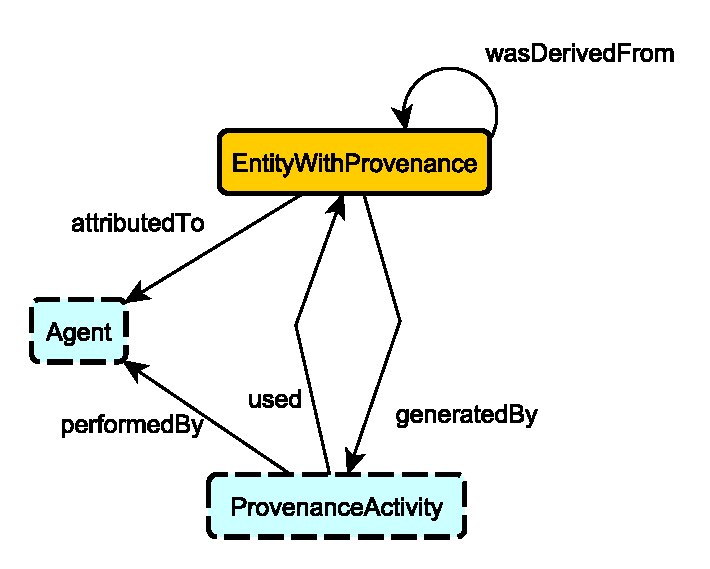
\includegraphics[width=.7\textwidth]{figures/provenance}
\end{center}
\caption{Schema Diagram for the Provenance Pattern. The visual notation is explained in Chapter \ref{chap:prelims}.}
\label{fig:Provenance}
\end{figure}
\subsection{Summary}
\label{sum:Provenance}
%%%%%%%%%%%%%%%%%%%%%%%%%%%%
The \textsf{EntityWithProvenance} Pattern is extracted from the PROV-O ontology. At the pattern level, we do not want to make the ontological committment to a full-blown ontology. It suffices to align a sub-pattern to the core of PROV-O \cite{provo}.

The \textsf{EntityWithProvenance} class is any item of interest to which a developer would like to attach provenance information. That is they are interested in capturing, who or what created that item, what was used to derive it, and what method was used to do so. The ``who or what'' is captured by using the \textsf{Agent} class. The property, \textsf{wasDerivedFrom} is eponymous---it denotes that some set of resources was used during the \textsf{ProvenanceActivity} to generate the \textsf{EntityWithProvenance}.

%%%%%%%%%%%%%%%%%%%%%%%%%%%%%%%%%%%%%%%%%%%%%%%%%%%%%%%%
\subsection{Axiomatization}
\label{axs:Provenance}
%%%%%%%%%%%%%%%%%%%%%%%%%%%%
\begin{align}
\exists\textsf{attributedTo}.\textsf{Agent} &\sqsubseteq \textsf{EntityWithProvenance}\\
\textsf{EntityWithProvenance} &\sqsubseteq \forall\textsf{attributedTo}.\textsf{Agent}\\
\exists\textsf{generatedBy}.\textsf{ProvenanceActivity} &\sqsubseteq \textsf{EntityWithProvenance}\\
\textsf{EntityWithProvenance} &\sqsubseteq \forall\textsf{generatedBy}.\textsf{ProvenanceActivity}\\
\exists\textsf{used}.\textsf{EntityWithProvenance} &\sqsubseteq \textsf{ProvenanceActivity}\\
\textsf{ProvenanceActivity} &\sqsubseteq \forall\textsf{used}.\textsf{EntityWithProvenance}\\
\exists\textsf{performedBy}.\textsf{Agent} &\sqsubseteq \textsf{ProvenanceActivity}\\
\textsf{ProvenanceActivity} &\sqsubseteq \forall\textsf{performedBy}.\textsf{Agent}
\end{align}

%%%%%%%%%%%%%%%%%%%%%%%%%%%%%%%%%%%%%%%%%%%%%%%%%%%%%%%%
\subsection{Explanations}
\label{exp:Provenance}
%%%%%%%%%%%%%%%%%%%%%%%%%%%%
\begin{enumerate}
\item Scoped Domain:The scoped domain of \textsf{attributedTo}, scoped by \textsf{Agent}, is \textsf{EntityWithProvenance}.
\item Scoped Range: The scoped range of \textsf{attributedTo}, scoped by \textsf{EntityWithProvenance}, is \textsf{Agent}. 
\item Scoped Domain:The scoped domain of \textsf{generatedBy}, scoped by \textsf{ProvenanceActivity}, is \textsf{EntityWithProvenance}.
\item Scoped Range: The scoped range of \textsf{generatedBy}, scoped by \textsf{EntityWithProvenance}, is \textsf{ProvenanceActivity}.
\item Scoped Domain:The scoped domain of \textsf{used}, scoped by \textsf{EntityWithProvenance}, is \textsf{ProvenanceActivity}
\item Scoped Range: The scoped range of \textsf{used}, scoped by \textsf{ProvenananceActivity}, is \textsf{EntityWithProvenance}.
\item Scoped Domain:The scoped domain of \textsf{performedBy}, scoped by \textsf{Agent}, is \textsf{ProvenanceActivity}.
\item Scoped Range: The scoped range of \textsf{performedBy}, scoped by \textsf{ProvenanceActivity}, is \textsf{Agent}.
\end{enumerate}

%%%%%%%%%%%%%%%%%%%%%%%%%%%%%%%%%%%%%%%%%%%%%%%%%%%%%%%%
\subsection{Competency Question}
\label{cqs:Provenance}
%%%%%%%%%%%%%%%%%%%%%%%%%%%%
\begin{enumerate}[CQ1.]
\item temporary item
\end{enumerate}

\newpage
%%%%%%%%%%%%%%%%%%%%%%%%%%%%%%%%%%%%%%%%%%%%%%%%%%%%%%%%
% End Section
%%%%%%%%%%%%%%%%%%%%%%%%%%%%%%%%%%%%%%%%%%%%%%%%%%%%%%%%
%%%%%%%%%%%%%%%%%%%%%%%%%%%%%%%%%%%%%%%%%%%%%%%%%%%%%%%%